\documentclass[mathserif,xcolor=dvipsnames]{beamer}

\usepackage{pset}

\usepackage{graphicx}
\usepackage{amssymb}
\usepackage{mathtools}

\usetheme{Madrid}
\usecolortheme[named=RawSienna]{structure} 
\useoutertheme{umbcfootline} 
%\usetheme[height=7mm]{Rochester} 
\setbeamertemplate{items}[ball] 
\setbeamertemplate{blocks}[rounded][shadow=true] 
\setbeamertemplate{navigation symbols}{} 


\renewcommand*{\Z}{\mathbb{Z}}
\renewcommand*{\R}{\mathbb{R}}
\renewcommand*{\C}{\mathbb{C}}
\DeclareMathOperator*{\argmax}{arg max}

\title[The Geometry of DBNs]{The Geometry of Deep Belief Networks}
\author{Aaron Pribadi}
\institute[HMC]{Harvey Mudd College}
\date{September 20, 2011}

\begin{document}

\begin{frame}[plain]
    \maketitle
\end{frame}


\begin{frame}{Algebraic Statistics}
    The field of \textbf{algebraic statistics} examines statistical problems using
    the tools of algebraic geometry and commutative algebra.

    \linespace
    \begin{itemize}
    \item geometric (coordinate-invariant) point of view
    \item algorithms from computational algebra
    \end{itemize}
\end{frame}

\begin{frame}{Algebraic Geometry}
    What is \textbf{algebraic geometry}?
    \begin{center}
    ``geometry of polynomials'' \qquad $\longrightarrow$ \qquad more abstraction
    \end{center}

    \linespace
    A quote from David Mumford:

    \begin{quote}
    Algebraic geometry seems to have acquired the reputation of being esoteric,
    exclusive, and very abstract, with adherents who are secretly plotting to
    take over all the rest of mathematics. In one respect this last point is
    accurate.
    \end{quote}
\end{frame}

\begin{frame}{The Probability Simplex}
    Probability distribution over $[n] = \{1,2,\ldots, n\}$:
    \[
        p(k) = x_k,
        \qquad
        \text{where }
        \sum_k x_k = 1,
        \;
        x_k \ge 0.
    \]

    \pause
    
    
    The $(n-1)$-dimensional \textbf{probability simplex} is the space of
    distributions:
    \[
        \Delta_{n-1} = \cdil*{(x_1, \ldots, x_n) 
        \;\Bigl\vert\;
        \sum_k x_k = 1,\; x_k \ge 0}
        \subset
        \R^n.
    \]
\end{frame}

\begin{frame}
    \linespace
    \linespace
    \begin{center}
    \scalebox{0.5}{ 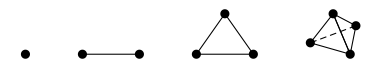
\includegraphics[scale=1]{simplices.png} }
    \end{center}
\end{frame}

\begin{frame}{Example: Independence Model}
    Two binary random variables:
    \[
        X = (X_1, X_2), \quad X \in \{0,1\}^2.
    \]
    Independence condition:
    \[
        p(X_1, X_2) = f(X_1)\;g(X_2)
    \]
\end{frame}

\begin{frame}{Example: Independence Model}
    Let $p_{ij} = p(i,j)$. A distribution $(p_{00}, p_{01}, p_{10}, p_{11})$
    is a point in $\Delta_3$.

    \linespace
    Polynomial constraints (for independence):
    \[
        f_{ij} = p_{ij} - (p_{i0} + p_{i1}) (p_{0j} + p_{1j}) = 0
        \qquad
        \text{for all }i,j.
    \]
    The independence model is the subset of $\Delta_3$ satisfying the above
    polynomial equations:
    \[
        \mathcal{M} = \Delta_3 \cap \{p  \mid f_{ij} = 0 \quad\forall\; i,j\}.
    \]
\end{frame}

\begin{frame}{Restricted Boltzmann Machine (RBM)}
    Model over visible nodes $v \in \{0,1\}^n$ and hidden nodes $h \in
    \{0,1\}^k$.
    \begin{center}
    \scalebox{0.7}{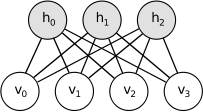
\includegraphics{rbm.png}}
    \end{center}
    \vspace{-0.5cm}
    Energy of a state :
    \[
        H(v, h) = h^T W v  + b^T v + c^T h
        \qquad
        \text{\scriptsize ($W$ is a matrix, $b$ and $c$ are vectors.)}
    \]
    Probability of a state:
    \[
        p(v, h) = \frac 1 Z \exp\sdil[\Big]{-H(v, h)}
        \qquad\qquad
        \text{\scriptsize ($Z$ is a normalizing constant)}
        \qquad
    \]
\end{frame}

\begin{frame}{Restricted Boltzmann Machine (RBM)}
    Since some nodes are hidden, we can \textbf{marginalize} over the hidden
    states:
    \[
        p(v) = \sum_{h \in \{0,1\}^k} p(v, h)
    \]

    \pause

    Given some sample values $\cdil*{v^{(i)} \in \{0,1\}^n}$, we can fit the
    weights $W, b, c$ by \textbf{maximum-likelihood}:
    \[
        \argmax_{W, b, c}\; \prod_{i} p\pdil*{v^{(i)}}
    \]
\end{frame}

\begin{frame}{Deep Belief Network (DBN)}
    \begin{itemize}
    \item Machine Learning
    \item `Deep Learning'
    \item MNIST dataset\\
    \begin{center}
    \scalebox{0.8}{
    
\includegraphics{./mnist_0.png}\,
    
\includegraphics{./mnist_1.png}\,
    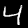
\includegraphics{./mnist_2.png}\,
    
\includegraphics{./mnist_3.png}\,
    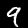
\includegraphics{./mnist_4.png}
    }
    \end{center}
    \end{itemize}
\end{frame}

\begin{frame}{Deep Belief Network (DBN)}
    \begin{columns}[T]
    \begin{column}{0.6\textwidth}
    A DBN has RBMs `stacked' together.

    \begin{itemize}
    \item Fit a RBM to the input data.
    \item Input values correspond to values in the hidden row above.
    \item Use the transformed data to train the next RBM.
    \item Repeat for all rows.
    \item At the top, fit with both input values and classification values.
    \end{itemize}

    \end{column}

    \begin{column}{0.3\textwidth}
    \begin{center}
    \scalebox{0.6}{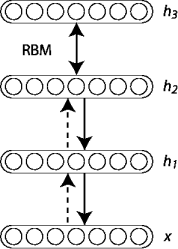
\includegraphics{DBN3.png}}
    \end{center}
    \end{column}
    \end{columns}
\end{frame}

\begin{frame}{Prior Work}
    Cuerto, Morton, Sturmfels:\\
    \begin{itemize}
    \item[] The (Zariski closure of the) RBM with one hidden node is the first
    secant variety of the Segre variety of projective lines.  RBMs with more
    hidden nodes are obtained by taking Hadamard powers.

    \item[] The variety's dimension is the full $nk + n + k$ (for certain parameters).
    \end{itemize}

    Ay, Montufar:\\
    \begin{itemize}
    \item[] It is possible to construct a DBN with $\frac{2^n}{2(n-b)}$ hidden
    layers of width $n$ (where $b \sim \log n$) capable of approximating any
    distribution on $\{0,1\}^n$ arbitrarily well.
    \end{itemize}

\end{frame}

\begin{frame}{Goals}
    \begin{itemize}
    \item An algebro-geometric viewpoint on DBNs
    \item Sharper bounds on universal approximation for RBMs and DBNs
    \item Bonus: Efficient optimization on DBNs (or other graphical models)
    \end{itemize}
\end{frame}

\begin{frame}{Credits}
    The image of simplices is
    \begin{center}
    {\scriptsize
    Copyright \textcopyright\, 2005--2011, The Sage Development Team. 
    }
    \end{center}
    The images for the RBM and DBN are
    \begin{center}
    {\scriptsize
    Copyright \textcopyright\, 2008--2009, Theano Development Team. All rights reserved.
    }
    \end{center}
\end{frame}

\begin{frame}{References}
\begin{thebibliography}{100}
    \bibitem{RBM} Cueto, Morton, Sturmfels. ``Geometry of the Restricted
    Boltzmann Machine''.  2009.
     \bibitem{RBM2} Ay, Montufar.  ``Refinements of Universal Approximation
     Results for Deep Belief Networks and Restricted Boltz mann Machines''.
     2011.
    \bibitem{A3} Drton, Sturmfels, Sullivant. \textit{Lectures on Algebraic
    Statistics}. 2009.
    \bibitem{A8} Hinton.  ``A fast algorithm for deep belief nets''.  2007.
\end{thebibliography}

\end{frame}
    

\end{document}
